\chapter{Introduction}

\dictum[Теодо́сій Григо́рович Добжа́нський (Theodosius
Dobzhansky)\footnotemark]{Nothing in biology makes sense […]}
\footnotetext{\citet{Dobzhansky:1973}}

\section{The central dogma}

% <<<
At the core of every living being is its genetic inheritance. The genetic
inheritance is what is being passed down from parents to their offspring, and
contains a blueprint detailing how to construct a new individual from a single
cell in a process called \define{embryogenesis}. This genetic inheritance is
physically present in the form of \dna in almost every living cell.\footnote{And
to some extent in non-living particles called \define{viruses}.}

As a medium of information storage, \dna is complemented by two other types of
molecules in the cell that, respectively, carry out the instructions encoded in
the \dna by performing specific biochemical functions, and serve as an
intermediary between information storage and execution. The intermediaries,
which are called \define{\rna}, copy out specific parts of the complete
instructions from the \dna and carry them to factories which translate the
instructions into highly specialised machines. These machines are called
\define{proteins}. The \define{central dogma of molecular biology} states that
information is thus transmitted from \dna to \rna, and from \rna to proteins,
but never from proteins back to \rna or \dna (\cref{fig:central-dogma})
\citep{Crick:1958,Crick:1970}. When first published, the central dogma concisely
summarised the available evidence at the time. Now, more than half a century
later, this still largely holds true.

\textfig{central-dogma}{body}{0.75\textwidth}
    {The central dogma of molecular biology.}{The solid arrows represent
    observed transfers of information; the dashed arrows represent what
    \citet{Crick:1970} referred to as “potential” transfers; today we know that
    the transfer \(\text{\rna}\rightarrow\text{\dna}\) does in fact occur under
    certain circumstances; the transfer \(\text{\dna}\rightarrow\text{protein}\)
    has still not been observed. Notably, the \emph{absent} transfers in the
    original publication are still considered non-existent.}

The very high-level view of the central dogma was complemented by a detailed
mechanistic description over the years, and these efforts are still ongoing.
This thesis investigates one minute aspect concerning the translation of \rna
into proteins. To better explain how it fits into the general picture of the
central dogma, we first need to understand its leading actors and their
interplay. The three main roles are fulfilled by \dna, \rna and proteins,
respectively, and we are now going to take a look at all of them in turn.
% >>>

\subsection{\abbr{dna}}

% <<<
\dna consists of a long chain of \define[{\defineword{nucleotide} molecule
consisting of a ribose, one or more phosphate groups and a nucleobase (example:
cytidine monophosphate, a nucleotide of cytosine)\footnotemark\\%
\marginfig{nucleotide}}]{nucleotides}\footnotetext{Figure adapted from
\url{https://commons.wikimedia.org/w/index.php?title=File:Nucleotides_1.svg&oldid=128814238}}.
The chemical structure of nucleotides enables them to polymerise into long,
relatively stable chains. \dna is made up of nucleotide monomers, which contain
any of four different types of nucleobases: adenine (\nA), cytosine (\nC),
guanine (\nG) and thymine (\nT). Thus, \dna can be thought of as a long string
of four different letters, and that is indeed how it is often represented. Text
is written from left to right in Western cultures. By convention, \dna is
written from \fivep to \threep.\footnote{The numbers are referring to the
numbering of the carbon atoms in each nucleotide’s ribose, which form covalent
bonds in the \dna so that the \fivep carbon atom is exposed at one end of the
chain, and the \threep end is exposed at the other.}

\dna is present in the cell in the form of double-stranded helices: each \dna
molecule consists of two paired chains, wound tightly around each other, with
the bases on each chain pairing up such that every \nA on one chain is paired
with a \nT on the other, and each \nC is paired with a \nG. This striking
symmetry is known as Watson–Crick base pairing, after its discoverers
\citep{Watson:1953}. Thus, \dna is made up of two complementary strands,
redundantly holding the genetic information. This redundancy is used in \dna
copying (which occurs at every cell division, and is the mechanism by which
genetic information is passed from one cell to its offspring) to synthesise two
newly formed \dna molecules, of which each contains one strand of the parent
\dna molecule (\define{semiconservative replication}).

The information on the \dna is not stored in one consecutive piece. Rather, \dna
consists of relatively short stretches encoding a specific function, separated
by long stretches that do not directly encode any function. The “function” is
what is transmitted, as per the central dogma, to \rna and, in many cases, on to
proteins. Such self-contained, functional stretches are called
\define[\defineword{gene} self-contained stretch of \abbr{dna} that is
transcribed to perform a function]{genes}. To perform its function, a gene has
to be transcribed into a catalytically active form, the \rna.\todo[ref]{Human Genome Project}
% >>>

\subsection{\abbr{rna}}

% <<<
\rna is the product of transcription of a gene from \dna. Unlike the latter,
\rna is created as a single strand. This has two consequences: First, \rna is
much less stable than \dna, and slowly degrades. \rna thus has a finite
life-time, and the pool of \rna must be replenished by continuous transcription.
Second, single-stranded ribonucleic acid spontaneously changes its spatial
conformation by forming Watson--Crick base pairs between nucleotides in its own
sequence, where this is \define[\defineword{steric effect} atoms occupy discrete
space and cannot overlap]{sterically} possible (i.e.\ where forming such a bond
does not require bending the chain too much to “snap” it). The resulting
structure can have functional consequences for the \rna. Because the structure
is determined by, and exists on a higher level than the sequence identity of the
\rna, it is called \define{secondary structure}.

Another difference between \dna and \rna is the use of slightly different
nucleotides: instead of \nT, \rna uses \nU (uracil), which, like \nT, base-pairs
with \nA. Despite the fact that the genetic information is encoded in virtually
the same way in \dna and \rna, transcription of \dna into \rna requires a
complex machinery. The core of this machinery is a complex enzyme called an
\define{\rna polymerase}. In eukaryotes, three different, evolutionarily related
\rna polymerases (\pol1, \pol2 and \pol3) are responsible for transcribing
different types of \rna.

\rna performs numerous different functions, but one very important subcategory
of \rna does not perform any function on its own; rather, it is an intermediary
between the genetic information on the \dna and the final protein product, which
in turn performs cellular functions. This class of \rna is called \mrna.
\mrna[s] are the product of the transcription of protein-coding genes by \pol2.
By contrast, \rna[s] which are not protein-coding are denoted as \ncrna.
Transcription of \mrna requires an exquisite control, and many different \tf[s]
are known to regulate different genes in different cellular conditions. This
results in different \mrna genes being transcribed at highly different levels,
leading to several orders of magnitude of difference in \mrna abundance. Even
more strikingly, the same \mrna can be transcribed at different levels under
different conditions. \mrna is further processed in several steps before the
mature \mrna is exported from the cell’s nucleus into the cytoplasm, where it is
translated into proteins, and, over time, decays. Taken together, this leads to
very differentiated \mrna profiles under different conditions, which imbue the
cells with a unique phenotype. This forms the basis of cellular differentiation
into different cell types and tissues in multicellular eukaryotes.\todo{Introns?
Alternative splicing?}\todo[ref]{Berthelot, Ule}
% >>>

\subsection{Proteins}

% <<<
Proteins, finally, are the main effectors of cell function. Like \dna and \rna,
they consist of chains of smaller molecules, so-called
\define[{\defineword{amino acid} molecule consisting of an amino–carboxyl
backbone and a specific side-chain (example: valine)\\%
\marginfig{amino-acid}}]{amino acids}, which are strung together to form
\define{polypeptides}. Each amino acid is a small molecule with unique
properties which, jointly, shape the function of the final protein. Individual
amino acids are strung together in a chemical reaction that links a carboxyl
group covalently with an amino group on the next amino acid to form a
\define[\defineword{peptide bond} a covalent bond formed between a carboxyl and
an amino group: \ce{COOH + NH2 -> CO-NH + H2O}]{peptide bond}
\citep{Alberts:2002}. Polypeptides, like many \rna[s], form secondary structures
via non-covalent bonds between amino acids, which are a function of the amino
acid sequence. Beyond this, proteins form even higher order three-dimensional
conformations called tertiary structures. When multiple proteins aggregate into
a complex consisting of several subunits, we speak of quarternary structure.

All these different levels of spatial organisation of proteins lead to the
creation of highly complex structures from originally one-dimensional chains. It
is their intricate structure which allows them to perform precise tasks in the
cell. Because they are the work horses of the cells, proteins are highly
abundant, with some proteins being present million-fold at any given moment
\citep{Milo:2013}. This is only possible because a single gene is transcribed
multiple times at once, and each resulting \mrna can be translated several
times, and simultaneously, before being degraded. The path
\(\text{\dna}\rightarrow\text{\rna}\rightarrow\text{protein}\) thus facilitates
an amplification from a single gene copy to many orders of magnitudes more
copies of the resulting protein. Despite the fact that multiple protein copies
can be created from a single \mrna molecule, and that the number varies from
transcript to transcript, protein abundance is predominantly determined by the
abundance of \mrna[s] \citep{Li:2014,Jovanovic:2015,Csardi:2014}.
% >>>

\section{Transcription \& translation}

\subsection{Transcription}

% <<<
As mentioned, three different polymerases are responsible for transcribing
nuclear \dna into different types of \rna. The precise ways in which the
different polymerases transcribe genes into their \rna products differ but the
fundamental aspects of transcription are similar. In all cases, a
\define[\defineword{motif} pattern describing a family of short sequences which,
though variable, have some degree of similarity]{motif} in the \dna sequence
initiates binding of a number of \tf proteins to the \dna. Such motifs, called
\define{promoters}, are found in the immediate vicinity of the \tss of their
target genes --- either upstream of the \tss or following closely after it,
inside the gene body. Once the \tf[s] have bound to the \dna on top of the \tss,
a polymerase attaches to the \dna and is held in place by the \tf[s].
Subsequently, the polymerase pries the double strand apart and starts
synthesising a new strand of \rna which pairs complementary with one of the
strands on the \dna (the \define{template strand}). The new \rna[’s] sequence is
thus identical to the other \dna strand (the \define{coding strand}). The \rna
is produced in the direction \fivep--\threep, implying that the template strand
is read in the direction \threep--\fivep during transcription. Once the first
few nucleotides of the \rna have been synthesised, the polymerase disassociates
from the \tf proteins, and the polymerase starts moving along the gene body,
transcribing it as it goes (this may require the presence of other \tf[s] called
\define{activators}, which are recruited by \define{enhancer} motifs elsewhere
on the \dna).

\todo[inline]{Figure: Transcription}
% >>>

\subsection{Translation}

The process by which proteins are created from \mrna transcripts is more complex
than the 1:1 transcription of \dna into \rna, which after all use a common
alphabet to encode the information they carry. By contrast, the
\define{translation} of \mrna transcripts into proteins requires a code to
interpret the genetic information. This code is known as the \define{genetic
code}.

\subsubsection{The genetic code}

% <<<
There are \num{20} different amino acids that are encoded by just \num{4}
different nucleotides. To allow this, several nucleotides must be combined to
form a larger unit coding for an amino acid. In the universal genetic code,
shared by all known species, this is accomplished by grouping three consecutive
nucleotides together to form non-overlapping \define{codons} along the \mrna.
This results in \(4^3 = 64\) possible codons, vastly more than there are amino
acids. As a consequence, the genetic code is \define{degenerate}: most amino
acids can be encoded by more than a single codon.

Codons furthermore serve as control points by defining where the translated
sequence on the \mrna starts and ends. The codon \codon{AUG}, in addition to
encoding the amino acid methionine, also marks the start of the coding sequence.
Three codons do not encode any amino acid, and instead signal the stop of
translation (\codon{UAA}, \codon{UAG}, \codon{UGA}). As a consequence, every
coding sequence starts with \codon{AUG}, ends with one of the stop codons, and
has a length divisible by \num{3}. \Cref{tab:genetic-code} contains a tabular
representation of the genetic code, which is valid, with only minor variations,
for all three domains of life.

\begin{table}
    \centering
    \def\s{\footnotesize stop}
    \def\h#1#2{\multicolumn{1}{#1}{\abbrsc{#2}}}
    \begin{tabu} to \textwidth {@{}
            >{\collectcell\codon}l<{\endcollectcell}
            >{\collectcell\anticodon}l<{\endcollectcell}
            l @{\qquad}
            >{\collectcell\codon}l<{\endcollectcell}
            >{\collectcell\anticodon}l<{\endcollectcell}
            l @{\qquad}
            >{\collectcell\codon}l<{\endcollectcell}
            >{\collectcell\anticodon}l<{\endcollectcell}
            l @{\qquad}
            >{\collectcell\codon}l<{\endcollectcell}
            >{\collectcell\anticodon}l<{\endcollectcell}
            l @{}}
        \toprule
        % Nasty, hand-coded length values.
        \noalign{\vskip-4pt}
        \h{@{}l}{C} & \h{l}{A} & \h{l}{AA} &
        \h{@{}l}{C} & \h{l}{A} & \h{l}{AA} &
        \h{@{}l}{C} & \h{l}{A} & \h{l}{AA} &
        \h{@{}l}{C} & \h{l}{A} & \h{l@{}}{AA} \\[-2pt]
        \midrule
        UUU & AAA & Phe & UCU & AGA & Ser & UAU & ATA & Tyr & UGU & ACA & Cys \\
        UUC & GAA & Phe & UCC & GGA & Ser & UAC & GTA & Tyr & UGC & GCA & Cys \\
        UUA & TAA & Leu & UCA & TGA & Ser & UAA & TTA & \s  & UGA & TCA & \s \\
        UUG & CAA & Leu & UCG & CGA & Ser & UAG & CTA & \s  & UGG & CCA & Trp \\
        \addlinespace
        CUU & AAG & Leu & CCU & AGG & Pro & CAU & ATG & His & CGU & ACG & Arg \\
        CUC & GAG & Leu & CCC & GGG & Pro & CAC & GTG & His & CGC & GCG & Arg \\
        CUA & TAG & Leu & CCA & TGG & Pro & CAA & TTG & Gln & CGA & TCG & Arg \\
        CUG & CAG & Leu & CCG & CGG & Pro & CAG & CTG & Gln & CGG & CCG & Arg \\
        \addlinespace
        AUU & AAT & Ile & ACU & AGT & Thr & AAU & ATT & Asn & AGU & ACT & Ser \\
        AUC & GAT & Ile & ACC & GGT & Thr & AAC & GTT & Asn & AGC & GCT & Ser \\
        AUA & TAT & Ile & ACA & TGT & Thr & AAA & TTT & Lys & AGA & TCT & Arg \\
        AUG & CAT & Met & ACG & CGT & Thr & AAG & CTT & Lys & AGG & CCT & Arg \\
        \addlinespace
        GUU & AAC & Val & GCU & AGC & Ala & GAU & ATC & Asp & GGU & ACC & Gly \\
        GUC & GAC & Val & GCC & GGC & Ala & GAC & GTC & Asp & GGC & GCC & Gly \\
        GUA & TAC & Val & GCA & TGC & Ala & GAA & TTC & Glu & GGA & TCC & Gly \\
        GUG & CAC & Val & GCG & CGC & Ala & GAG & CTC & Glu & GGG & CCC & Gly \\
        \bottomrule
    \end{tabu}
    \tabcap{genetic-code}{The genetic code.}
        {Shown is each codon (“\abbrsc{C}”), its potential corresponding
        anticodon (“\abbrsc{A}”) and the three-letter abbreviation of the
        corresponding amino acid (“\abbrsc{AA}”). \codon{AUG}, in addition to
        encoding methionine, also signals the start of translation. Not all
        anticodons exist in all species (adapted from \citet{Dos_Reis:2004}).}
\end{table}

The translation of \mrna into proteins is assisted by a special apparatus called
the \define{ribosome}. Ribosomes are large complexes of proteins and \rrna,
forming two subunits. In eukaryotes, these subunits are the 40S and 60S subunit,
respectively. During translation initiation, the 40S subunit scans along an
\mrna transcript until it finds a signal sequence surrounding a start codon
\citep{Kozak:2002}. There it is joined by the 60S subunit. The assembled
ribosome then pulls the \mrna through a channel in its structure and
progressively translates the codons on the \mrna into amino acids, which are
chained together to form a nascent polypeptide chain.
% >>>

\subsubsection{\abbr{trna}}

% <<<
Individual codons are translated into their corresponding amino acid by aid of
adapter molecules carrying a specific amino acid, and which recognise the
matching codon. This codon recognition is possible because the adapter molecules
are themselves \abbr{rna}s, and the codon is matched via complementary base
pairing of a part of the \rna sequence termed the \define{anticodon}. These
adapter molecules are called \define[{
    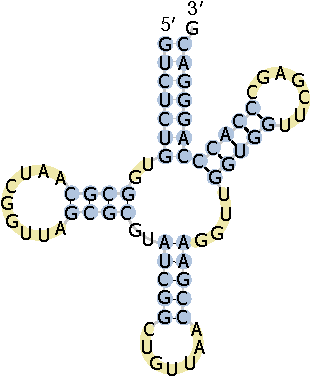
\includegraphics[width=\marginparwidth]{trna-asn}
    \figcapof{trna-asn}{\abbr{trna} secondary structure}{of a \trna coding
    for asparagine (Asn). Structure predicted by \name{COVE} \citep{Eddy:1994},
    rendered by \name{PseudoViewer 3} \citep{Byun:2009} and manually
    post-processed.}
}]{\trna}.

\trna[s] are encoded by small genes, around \SIrange{70}{90}{bp} in length.
Their transcription is driven by \pol3. Unlike for protein-coding genes, whose
promoters lie upstream of the actual gene body, the promoter is found
\emph{inside} a \trna gene, in two disjoint regions called the \define{A box}
and \define{B box}, respectively. The A box starts about \SI{10}{bp} downstream
from the \tss, whereas the B box can be found at a variable distance of about
\SIrange{30}{60}{bp} downstream from the A box. \trna transcription is initiated
when the transcription factor \tfiiic binds to the B box motif. \tfiiic leads to
the binding of the \pol3 recruitment factor \tfiiib upstream of the \trna gene.
A subunit of \tfiiib, the \tbp, binds to an upstream \seq{TATA} motif, if
present. Although the presence of this motif is not essential for \trna gene
transcription, it is in fact well conserved upstream of mammalian \trna genes,
suggesting a non-negligible effect on transcription. Bindin of \tfiiib in turn
leads to the association of \pol3 with the gene body, and the initiation of
transcription. Transcription stops when \pol3 encounters a short \nT repeat
downstream of the \trna gene \citep{Dieci:2007}.

\textfig{trna-gene}{body}{\textwidth}{\abbr{trna} gene transcription}
    {immediately before \pol3 is recruited. The A and B box are highlighted in
    \primaryname{} and \secondaryname{}, respectively. Diagram is not to scale.}

To avoid confusion, codons in this thesis will always be typeset like this:
\fwdstrand{\codon{CAU}}; anticodons will always be typeset like this:
\revstrand{\anticodon{ATG}} (the directionality is indicated here to clarify the
differences in reading direction between codons and anticodons; it will
generally be omitted in the remainder of the text).
% >>>

\section{\abbr{rnaseq} for the study of gene expression}

\section{\abbr{chipseq}}

\subsection{\abbr{chipseq} quantifies \abbr{trna} gene expression}

\section{Mouse development as a model system}

\section{Codon usage and anticodon abundance}

\todo[inline]{Description of the goals of the thesis}

Throughout this thesis I am going to use several related measures:

\begin{enumerate}
    \item codon usage,
    \item \rcu,
    \item anticodon abundance and
    \item \raa.
\end{enumerate}

The \define{codon usage} of a codon is the frequency with which this codon
occurs in a given transcriptome. This is either the raw number of occurrences in
the transcripts under consideration, or the number of occurrences, weighted by
the expression of each transcript.

The \define{anticodon abundance} of an anticodon is the amount of \trna
decoding a given anticodon, present in the cell at a given instance. Other
publications define the anticodon abundance in terms of \trna gene copy number;
however, in the context of this thesis, the anticodon abundance is usually
quantified by \trna gene expression, and is thus proportional to the number of
\trna molecules of each anticodon isoacceptor present in the cell.

The \define{\rcu} of a codon is that codon’s contribution to the amino acid it
codes for, relative to all other synonymous codons. The \rcu of all synonymous
codons sums to \num{1}.

The \define{\raa} of an anticodon is defined equivalently to the \rcu based on
the anticodon abundance. That is, the contribution of an anticodon to its amino
acid isotype, relative to the other anticodons in the same isotype.

In all of the above, I exclude the stop codons.

Several publications use the term \cub to describe divergence in codon usage
between different sets of genes within a genome, or differences between genomes.
The \cub is then equivalent either to the codon usage as defined in this thesis,
or the \rcu.

\section{Structure of this thesis}

\section{TO DOs}

\todo[inline]{\begin{enumerate}[noitemsep,nolistsep,leftmargin=*]
    \item Molecular and functional structure description of pol2 and pol3
    \item Structure of a tRNA gene (internal promoters etc.)
    \item tRNA modification, (re)loading and degradation: life-cycle has impact
        on abundance, and thus on translation efficiency. We completely ignore
        this; but why can we do this?
    \item Anticodon isoacceptors, tRNA genes, wobble base pairing
    \item tAI, codon usage, codon usage bias, anticodon abundance bias
    \item Tiny bit about mouse embryonology
    \item Prior research/literature review of tRNA and codon usage, also outside
        mammals!
\end{enumerate}}

\todo{Take intro from paper}

\subsection{Posttranscriptional modification}

In particular A-to-I conversion (deamination), which is relevant in tRNA gene
wobble base pairing!
% vim: fmr=<<<,>>>
